\subsubsection{Pattern Matching Verses Learning an Algorithm} \label{sec:theory-approach-methodology-pattern-matching-vs-learning-an-algorithm}

In the introduction to Section \ref{sec:theory-approach} we laid out our objectives from this research, namely to show that it is possible to improve the effectiveness of deep neural network models using symbols when training using an impoverished dataset and to also show that the presence of symbols allows the model to discover a general solution to the problem similar to how symbols affect the ability of humans to learn. In the previous two sections, we described the first stage of our theory development that aims to satisfy the first objective. Here we further develop our theory and attempt to satisfy the second objective by showing that without symbols the ability of neural networks to find a general solution to the problem is diminished.

\paragraph{Pattern Matching}

We explained in Section \ref{sec:theory-hypothesis} the concept of multi-task learning and described how the common representation shared by both the symbolic inputs and the noisy handwritten digits can make learning more effective. Learning from the noisy handwritten digits alone is difficult due to the high number of variations presented to the model. The presence of clear symbols guides the neural network to discover a good representation in its hidden weights, that can be used to identify the various noisy handwritten digits. The model then learns to perform a mapping or pattern matching between the digits and the desired outcome of the arithmetic operation.

\begin{figure}[t]
	\centering
	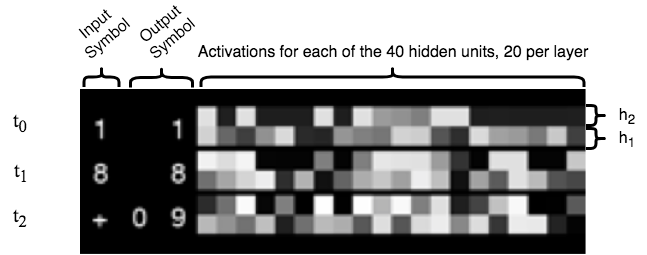
\includegraphics[max width=\textwidth]{activations-cluster}
	\caption{A visualization of hidden layer activations of a deep recurrent network with three time steps and two hidden layers 20 units each. The activations are the result of presenting the model with the operation: 1 + 8, in reverse Polish notation}
	\label{fig:activations-cluster}
\end{figure} 

To verify that this is indeed what is happening, we need to understand the relationship between the network's inputs and the state of its hidden layers. We therefore use a visualization technique, known as activations clustering, that captures the value of $h_t$ on each hidden layer and renders these as intensities in an image. The output value of each unit in the hidden recurrent layers is mapped to a pixel intensity where an output of -1 would map to 0 and an output of 1 would map to 255. Each unit would be assigned a region on the activations cluster. Figure \ref{fig:activations-cluster} shows an activations cluster for a recurrent network with three time steps and two hidden layers, 20 units each. Our expectation is that the clusters obtained from the model trained using symbols would show the consistency described above. This means that when the same combination of digits and operation is presented to the network, regardless of the instances of the MNIST digits used, a particular region of the cluster would show the same pattern. We also expect that when we contrast this behavior with that of a model trained without the presence of symbols, no such pattern would be apparent.

Besides observing this consistency in the hidden layer activations, we would expect to see some patterns emerge as well. For example, the ``carry one" concept that humans use to do complex addition and that forms an important function in binary arithmetic, might be represented in the network's hidden layers. Since discovering such patterns would be easier with clear symbols than with noisy handwritten digits, the presence of symbols should significantly improve the ability of the neural networks to achieve this goal. Consider the operations 8 + 1 and 8 + 2. The first does not produce a carry whereas the second does. We expect that by examining activations clusters produced for these two operations, we would observe a transition in some part of the network that indicates a carry being generated. Discovering this carry concept is a major step towards developing a learning system that is able to generalize in the same way humans can.

\paragraph{Learning an Algorithm}

To satisfy our second object, we would like to show that symbols help the learning process advance beyond the ability to do pattern matching effectively and instead actually learn the general algorithm that performs the arithmetic operation. Showing that this is the case would support the use of symbols in neural network learning analogous to their use in human learning, for example when children learn arithmetic as described in Section \ref{sec:theory-approach}. Our approach involves developing recurrent neural networks that are trained on only a subset of the dataset and then tested on the remaining examples in the dataset. We believe that without the presence of symbols it would be very difficult for an artificial neural network to perform well, just like human learners that learn without the knowledge shared by other agents. By providing symbols during training, our models should be able to generalize to the unseen examples and therefore show that an algorithm has been developed.
